

%% AAPT Physics Bowl Exams Questions
%%----------------------------------------


%% this section contains 23 problems


%% PhysicsBowl 2015
%%----------------------------------------
\element{aapt}{ %% Bowl-A6
\begin{question}{bowl-2015-q35}
    Two uniform disks, $X$ and $Y$, have equal masses, $M$,
        but different radii such that $r_X < r_Y$.
    Both disks initially are at rest.
    A force $F$ is applied tangent to each disk at its right edge for the same amount of time.
    \begin{center}
    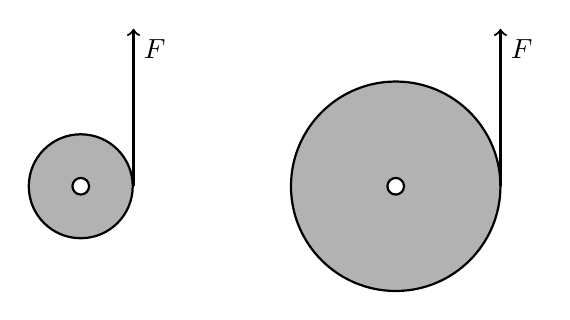
\begin{tikzpicture}
        \draw[thick,fill=white!70!black] (-2,0) circle (0.66);
        \draw[thick,fill=white] (-2,0) circle (3pt);
        \draw[thick,->] (-1.33,0) -- ++ (90:2cm)
            node[pos=1.0,anchor=north west] {$F$};
        \draw[thick,fill=white!70!black] (+2,0) circle (1.33);
        \draw[thick,fill=white] (+2,0) circle (3pt);
        \draw[thick,->] (3.33,0) -- ++ (90:2cm)
            node[pos=1.0,anchor=north west] {$F$};
    \end{tikzpicture}
    \end{center}
    As a result, each disk rotates counterclockwise in the plane
        of the page about a fixed frictionless axis through its center.
    Which one of the following choices correctly compares the
        magnitudes of angular momentum $L$ about the center axis and
        total kinetic energy $K$ of disk $X$ and disk $Y$?
    \begin{choices}
        \wrongchoice{$L_x<L_y$; $K_X<K_Y$}
        \wrongchoice{$L_x<L_y$; $K_X>K_Y$}
        \wrongchoice{$L_x=L_y$; $K_X=K_Y$}
        \wrongchoice{$L_x=L_y$; $K_X<K_Y$}
      \correctchoice{$L_x<L_y$; $K_X=K_Y$}
    \end{choices}
\end{question}
}

\element{aapt}{ %% Bowl-A6
\begin{question}{bowl-2015-q46}
    A uniform rod of mass $M$ and length $L$ is fixed to rotate about a
        frictionless pivot located $\frac{L}{3}$ from one end.
    The rod is released from rest incrementally away from being perfectly vertical,
        resulting in the rod rotating clockwise about the pivot.
    \begin{center}
    \begin{tikzpicture}
        \draw[thick] (0,-1) -- (0,2);
        \draw[fill] (0,0) circle (2pt) node[label distance=1em,pin=45:pivot] {};
        \node[anchor=west] at (0,-0.5) {$\dfrac{L}{3}$};
        \draw[thick,dashed,->] (0,-1) arc (270:240:1cm);
        \draw[thick,dashed,->] (0,2) arc (90:60:2cm);
    \end{tikzpicture}
    \end{center}
    When the rod is horizontal,
        what is the magnitude of the tangential acceleration of its center of mass?
    \begin{multicols}{3}
    \begin{choices}
        \wrongchoice{$\dfrac{1}{6} g$}
        \wrongchoice{$\dfrac{1}{2} g$}
        \wrongchoice{$\dfrac{4}{3} g$}
        \wrongchoice{$\dfrac{2}{3} g$}
      \correctchoice{$\dfrac{1}{4} g$}
    \end{choices}
    \end{multicols}
\end{question}
}


%% PhysicsBowl 2014
%%----------------------------------------
\element{aapt}{ %% Bowl-A6
\begin{question}{bowl-2014-q23}
    Two small identical coins (labeled $X$ and $Y$) are at rest on a horizontal disk rotating at a constant rate about an axis perpendicular to the plan of the disk and through its center.
    \begin{center}
    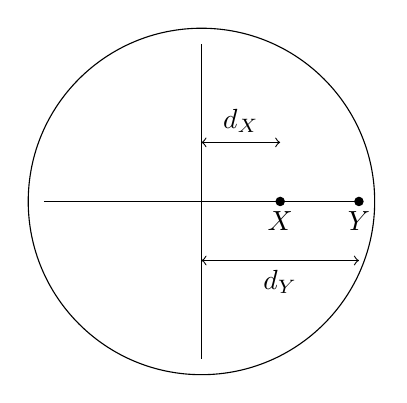
\begin{tikzpicture}
        \draw (0,0) circle (2.2cm);
        %% Axis
        \draw (0,-2) -- (0,+2);
        \draw (-2,0) -- (+2,0);
        %% Lables X and Y
        \draw[fill] (+1,0) circle (1.5pt) node[anchor=north] {$X$};
        \draw[fill] (+2,0) circle (1.5pt) node[anchor=north] {$Y$};
        %% Distances
        \draw[<->] (0,0.75) -- (1,0.75) node[pos=0.5,anchor=south] {$d_X$};
        \draw[<->] (0,-0.75) -- (2,-0.75) node[pos=0.5,anchor=north] {$d_Y$};
    \end{tikzpicture}
    \end{center}
    The distance of the coins from the center of disk is related by $d_X=\frac{1}{2} d_Y$.
    Which one of the following choices correctly identifies the relationship between $f_X$ and $f_Y$,
        the frictional force on coin $X$ and on coin $Y$, respectively?
    \begin{multicols}{2}
    \begin{choices}
        \wrongchoice{$f_X = \dfrac{1}{4} f_Y$}
      \correctchoice{$f_X = \dfrac{1}{2} f_Y$}
        \wrongchoice{$f_X = f_Y$}
        \wrongchoice{$f_X = 2 f_Y$}
        \wrongchoice{$f_X = 4 f_Y$}
    \end{choices}
    \end{multicols}
\end{question}
}

\element{aapt}{ %% Bowl-A6
\begin{question}{bowl-2014-q39}
    Two uniform disks, $X$ and $Y$, have masses $m_X < m_Y$, equal radii,
        and equal initial non-zero kinetic energies.
    \begin{center}
    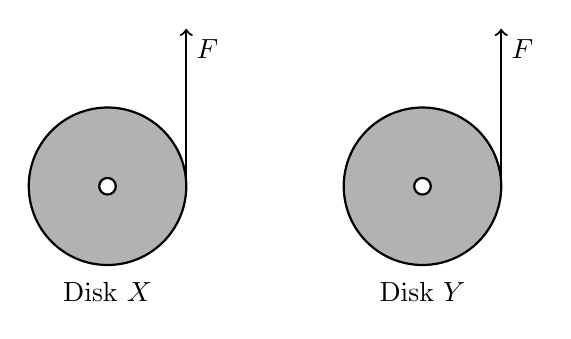
\begin{tikzpicture}
        %% Disk X, on left
        \draw[thick,fill=white!70!black] (-2,0) circle (1.00);
        \draw[thick,fill=white] (-2,0) circle (3pt);
        \draw[thick,->] (-1.00,0) -- ++ (90:2cm)
            node[pos=1.0,anchor=north west] {$F$};
        \node[anchor=north] at (-2,-1.10) {Disk $X$};
        %% Disk Y, on right
        \draw[thick,fill=white!70!black] (+2,0) circle (1.00);
        \draw[thick,fill=white] (+2,0) circle (3pt);
        \draw[thick,->] (3.00,0) -- ++ (90:2cm)
            node[pos=1.0,anchor=north west] {$F$};
        \node[anchor=north] at (+2,-1.10) {Disk $Y$};
    \end{tikzpicture}
    \end{center}
    Each disk rotates counterclockwise in the plane of the page about a
        fixed edge for the same amount of time.
    After the forces are applied, let $L$ represent the magnitude of the
        angular momentum about the center of a disk and $K$ represent the
        kinetic energy of a disk.
    Which one of the following choices correctly compares these quantities
        for disk $X$ and disk $Y$?
    \begin{choices}
        \wrongchoice{$L_X>L_Y$; $K_X<K_Y$}
        \wrongchoice{$L_X>L_Y$; $K_X>K_Y$}
        \wrongchoice{$L_X=L_Y$; $K_X=K_Y$}
        \wrongchoice{$L_X<L_Y$; $K_X<K_Y$}
      \correctchoice{$L_X<L_Y$; $K_X>K_Y$}
    \end{choices}
\end{question}
}

\element{aapt}{ %% Bowl-A6
\begin{question}{bowl-2014-q43}
    A long rod of length $L$ is pivoted about its left end.
    It is released from an angle $\theta$ above the horizontal.
    \begin{center}
    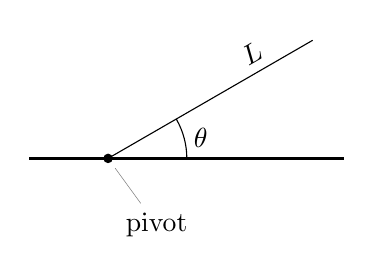
\begin{tikzpicture}
        \draw[line width=1.2pt] (-1,0) -- (3,0);
        \draw[fill] (0,0) circle (1.5pt) node[pin=280:pivot] {};
        \draw (0,0) -- ++ (30:3) node[pos=0.75,anchor=south,rotate=30] {$L$};
        \draw (0:1cm) arc (0:30:1cm) node[pos=0.5,anchor=west] {$\theta$};
    \end{tikzpicture}
    \end{center}
    What is the magnitude of the angular acceleration of the rod about the pivot when the rod is released?
    \begin{multicols}{3}
    \begin{choices}
        \wrongchoice{$\dfrac{6g}{L}\cos\theta$}
        \wrongchoice{$\dfrac{6g}{L}\sin\theta$}
        \wrongchoice{$\dfrac{3g}{L}\sin\theta$}
      \correctchoice{$\dfrac{3g}{L}\cos\theta$}
        \wrongchoice{$\dfrac{3g}{L}\sin\theta$}
    \end{choices}
    \end{multicols}
\end{question}
}

\element{aapt}{ %% Bowl-A6
\begin{question}{bowl-2014-q49}
    A solid, uniform disk of mass $M$ and radius $R$ rotates clockwise about its center with an angular speed $\omega_0$.
    \begin{center}
    \begin{tikzpicture}
        %% Surface
        \draw (-2,0) -- (2,0);
        \node[anchor=north,pattern=north east lines,minimum width=4cm,minimum height=0.05cm] at (0,0) {};
        %% Circle
        \draw (0,1) circle (1cm);
        \draw[thick,->] (0,1) -- ++ (225:1cm) node[pos=0.5,anchor=south east] {$R$};
        \draw[thick,->] (0,1) ++ (125:0.5cm) arc(125:-45:0.5cm);
        \draw (0,1) ++ (135:1.1cm) node[anchor=south] {$M$};
    \end{tikzpicture}
    \end{center}
    The disk then is placed onto a horizontal surface and beings moving only to the right, slipping as it rolls.
    The coefficient of friction between the floor and the disk is $\mu$ and the frictional force is considered constant throughout the motion.
    What is the angular speed of the disk when the disk starts rolling without slipping?
    \begin{multicols}{3}
    \begin{choices}
        \wrongchoice{$\dfrac{\mu}{2}\omega_0$}
        \wrongchoice{$\dfrac{1}{2}\omega_0$}
      \correctchoice{$\dfrac{1}{3}\omega_0$}
        \wrongchoice{$\dfrac{2\mu}{3}\omega_0$}
        \wrongchoice{$\dfrac{3}{5}\omega_0$}
    \end{choices}
    \end{multicols}
\end{question}
}


%% PhysicsBowl 2013
%%----------------------------------------
\element{aapt}{ %% Bowl-A6
\begin{question}{bowl-2013-q23}
    A small object of mass \SI{11.0}{\gram} is at rest \SI{30.0}{\centi\meter} from a horizontal disk's center.
    The disk starts to rotate from rest about its center with a constant angular acceleration of \SI{4.50}{\radian\per\second\squared}.
    What is the magnitude of the net force acting on the object after a time of $t=\SI{1/3}{\second}$ if the object remains at rest with respect to the disk?
    \begin{multicols}{2}
    \begin{choices}
        \wrongchoice{\SI{0}{\newton}}
        \wrongchoice{\SI{7.43e-3}{\newton}}
        \wrongchoice{\SI{1.49e-2}{\newton}}
      \correctchoice{\SI{1.66e-2}{\newton}}
        \wrongchoice{\SI{2.23e-2}{\newton}}
    \end{choices}
    \end{multicols}
\end{question}
}

\newcommand{\BowlTwentyThirteenQThirtyNine}{
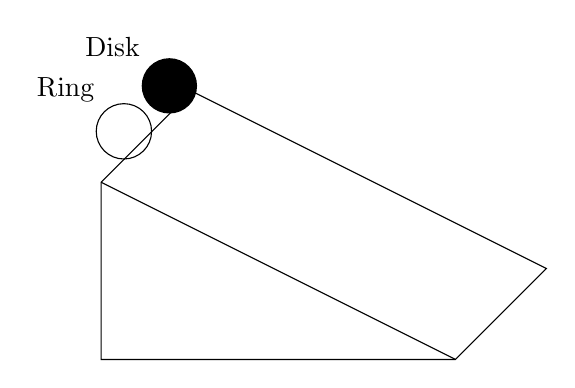
\begin{tikzpicture}[scale=0.75]
    %% Draw three dimensional wedge
    \draw (0,0,0) -- (6,0,0) -- (6,0,-4) -- (0,3,-4) -- (0,3,0) -- cycle;
    \draw (0,3,0) -- (6,0,0);
    %% Disk
    \node[anchor=south,circle,minimum size=2em,fill] (D) at (0,3,-3) {};
    \node[anchor=south east] at (D.north west) {Disk};
    %% Ring
    \node[anchor=south,circle,minimum size=2em,draw] (R) at (0,3,-1) {};
    \node[anchor=south east] at (R.north west) {Ring};
\end{tikzpicture}
}

\element{aapt}{ %% Bowl-A6
\begin{question}{bowl-2013-q39}
    An ideal uniform solid disk and an ideal uniform ring each have mass $M$ and radius $R$.
    Each object beings purely rolling without slipping down a rough inclined plane.
    The coefficients of friction for the disk and ring with the incline are $\mu_{disk}>\mu_{ring}$.
    \begin{center}
        \BowlTwentyThirteenQThirtyNine
    \end{center}
    As each object rolls down the incline,
        which statement is correct about the force of friction from the incline on the objects?
    \begin{choices}
      \correctchoice{The ring experiences a greater force of friction than the disk.}
        \wrongchoice{The disk experiences a greater force of friction than the ring.}
        \wrongchoice{The force of friction is equal and non-zero for both objects.}
        \wrongchoice{The force of friction is equal to zero for both objects.}
        \wrongchoice{Nothing can be concluded about the force of friction without more information.}
    \end{choices}
\end{question}
}

\element{aapt}{ %% Bowl-A6
\begin{question}{bowl-2013-q40}
    An ideal uniform solid disk and an ideal uniform ring each have mass $M$ and radius $R$.
    Each object beings purely rolling without slipping down a rough inclined plane.
    The coefficients of friction for the disk and ring with the incline are $\mu_{disk}>\mu_{ring}$.
    \begin{center}
        \BowlTwentyThirteenQThirtyNine
    \end{center}
    As the objects roll,
        what is the ratio of the ring's angular acceleration to the disk's angular acceleration calculated about an axis perpendicular to the objects face and through its center of mass?
    \begin{multicols}{3}
    \begin{choices}
        \wrongchoice{$1:2$}
        \wrongchoice{$2:1$}
        \wrongchoice{$\mu_{disk}:\mu_{ring}$}
        \wrongchoice{$4:3$}
      \correctchoice{$3:4$}
    \end{choices}
    \end{multicols}
\end{question}
}

\element{aapt}{ %% Bowl-A6
\begin{question}{bowl-2013-q47}
    Which one of the following choices best represents the magnitude of the angular momentum of the Earth associated with its rotation about its axis?
    \begin{multicols}{2}
    \begin{choices}
        \wrongchoice{\SI{e38}{\kilo\gram\meter\squared\per\second\squared}}
      \correctchoice{\SI{e34}{\kilo\gram\meter\squared\per\second\squared}}
        \wrongchoice{\SI{e30}{\kilo\gram\meter\squared\per\second\squared}}
        \wrongchoice{\SI{e26}{\kilo\gram\meter\squared\per\second\squared}}
        \wrongchoice{\SI{e22}{\kilo\gram\meter\squared\per\second\squared}}
    \end{choices}
    \end{multicols}
\end{question}
}


%% PhysicsBowl 2012
%%----------------------------------------
\element{aapt}{ %% Bowl-A6
\begin{question}{bowl-2012-q11}
    A girl twirls a small mass connected to the end of a string
        counterclockwise in a horizontal circle above her head.
    \begin{center}
    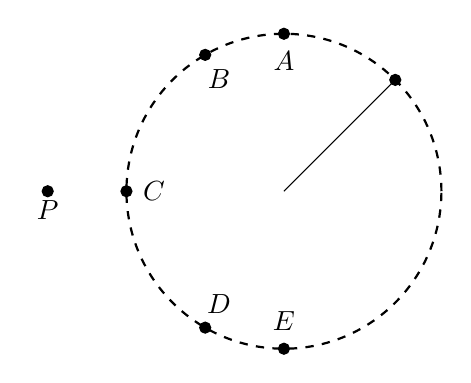
\begin{tikzpicture}
        \draw[thick,dashed] (0,0) circle (2cm);
        \draw (0,0) -- ++ (45:2cm);
        \draw[fill] (45:2cm) circle (2pt);
        %% Options
        \foreach \x/\y in {90/A,120/B,180/C,240/D,270/E}
            \draw[fill] (\x:2cm) circle (2pt) node[anchor=center,shift={(\x:-1em)}] {$\y$};
        %% Point P
        \draw[fill] (180:3cm) circle (2pt) node[anchor=north] {$P$};
    \end{tikzpicture}
    \end{center}
    The figure shows an outline of the mass's path viewed from
        above the twirling mass.
    If the girl needs the mass to pass through the point labeled
        $P$ in the figure, at which lettered point on the path
        should she let go of the string?
    \begin{multicols}{5}
    \begin{choices}
        \wrongchoice{$A$}
      \correctchoice{$B$}
        \wrongchoice{$C$}
        \wrongchoice{$D$}
        \wrongchoice{$E$}
    \end{choices}
    \end{multicols}
\end{question}
}

\element{aapt}{ %% Bowl-A6
\begin{question}{bowl-2012-q22}
    A girl swings a \SI{4.0}{\kilo\gram} mass with constant
        speed of \SI{3.24}{\meter\per\second} in a
        vertically-oriented circle of radius \SI{0.75}{\meter}.
    What is the net force acting on the mass when it is
        at the lowest point of the circle?
    \begin{multicols}{3}
    \begin{choices}
        \wrongchoice{\SI{96}{\newton}}
      \correctchoice{\SI{56}{\newton}}
        \wrongchoice{\SI{40}{\newton}}
        \wrongchoice{\SI{16}{\newton}}
        \wrongchoice{\SI{0}{\newton}}
    \end{choices}
    \end{multicols}
\end{question}
}

\element{aapt}{ %% Bowl-A6
\begin{question}{bowl-2012-q25}
    Which one of the following choices best represents
        the average angular speed of the hour hand on a standard clock?
    \begin{multicols}{2}
    \begin{choices}
        \wrongchoice{\SI{5.24e-1}{\radian\per\second}}
        \wrongchoice{\SI{2.62e-1}{\radian\per\second}}
        \wrongchoice{\SI{1.75e-3}{\radian\per\second}}
      \correctchoice{\SI{1.45e-4}{\radian\per\second}}
        \wrongchoice{\SI{7.27e-5}{\radian\per\second}}
    \end{choices}
    \end{multicols}
\end{question}
}

\element{aapt}{ %% Bowl-A6
\begin{question}{bowl-2012-q33}
    A solid, uniform sphere rolls without slipping on a floor
        along the $+x$-axis (to the right).
    \begin{center}
    \begin{tikzpicture}
        %% Floor and ball
        \draw[very thick] (-2,0) -- (4,0) node[pos=0.5,anchor=north,yshift=-1em] {Floor};
        \node[anchor=north,pattern=north east lines,minimum width=6cm] at (1,0) {};
        \node[anchor=south,circle,minimum size=0.75cm,draw,fill=white!50!black] at (-1,0) {};
        %% Axis labels
        \draw[thick,->] (2,1,0) -- (2,1,1) node[anchor=north] {$+z$};
        \draw[thick,->] (2,1,0) -- (3,1,0) node[anchor=west] {$+x$};
        \draw[thick,->] (2,1,0) -- (2,2,0) node[anchor=west] {$+y$};
    \end{tikzpicture}
    \end{center}
    The rotational kinetic energy associated with the sphere
        about an axis of rotation through its center of mass
        along the $+z$-axis (out of the plane of the page)
        is \SI{20}{\joule}.
    What is the translational kinetic energy associated with
        the sphere?
    \begin{multicols}{3}
    \begin{choices}
        \wrongchoice{\SI{8}{\joule}}
        \wrongchoice{\SI{10}{\joule}}
        \wrongchoice{\SI{20}{\joule}}
        \wrongchoice{\SI{40}{\joule}}
      \correctchoice{\SI{50}{\joule}}
    \end{choices}
    \end{multicols}
\end{question}
}

\element{aapt}{ %% Bowl-A6
\begin{question}{bowl-2012-q34}
    A mass $m$ attached to a light string of length $L$ is
        located at an angle $\theta$ below the horizontal as
        shown in the figure below.
    \begin{center}
    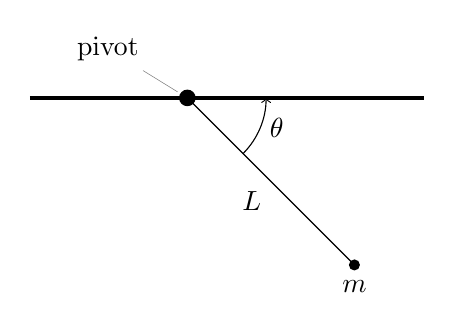
\begin{tikzpicture}
        %% horizontal
        \draw[ultra thick] (-2,0) -- (3,0);
        \fill (0,0) circle (3pt);
        \node[pin={145:pivot}] at (0,0) {};
        %% lighg string
        \draw[fill] (0,0) -- ++ (315:3)
            node[pos=0.5,anchor=north east] {$L$};
        %% mass 
        \fill (315:3) circle (2pt) node[anchor=north,yshift=-2pt] {$m$};
        \draw[->] (315:1) arc (315:360:1) node[pos=0.5,anchor=west] {$\theta$};
    \end{tikzpicture}
    \end{center}
    The mass then is released from rest.
    Calculated from an axis perpendicular to the plane of the
        page through the pivot, which one of the following
        choices represents the magnitude of the torque produced
        by the gravitational force acting on the mass at this instant?
    \begin{multicols}{2}
    \begin{choices}
        \wrongchoice{$mgL$}
        \wrongchoice{$mgL\sin\theta$}
      \correctchoice{$mgL\cos\theta$}
        \wrongchoice{$mgL\left(1-\sin\theta\right)$}
        \wrongchoice{$mgL\left(1-\cos\theta\right)$}
    \end{choices}
    \end{multicols}
\end{question}
}

\element{aapt}{ %% Bowl-A6
\begin{question}{bowl-2012-q43}
    Several forces act on a rigid body.
    If the resultant (net) force on the body is zero,
        which one of the following statements must be true?
    \begin{choices}
        \wrongchoice{The object is in translational equilibrium and rotational equilibrium.}
      \correctchoice{The object is in translational, but not necessarily rotational, equilibrium.}
        \wrongchoice{The object is in rotational, but not necessarily translational, equilibrium.}
        \wrongchoice{The object is in static equilibrium.}
        \wrongchoice{The object is in neither translational nor rotational equilibrium.}
    \end{choices}
\end{question}
}


%% PhysicsBowl 2011
%%----------------------------------------
\element{aapt}{ %% Bowl-A6
\begin{question}{bowl-2011-q35}
    Mary rides her bicycle directed due South.
    She applies the brakes quickly bringing the bicycle to rest with the wheels rolling without slipping on the group.
    Which one of the following choices best represents the direction of the angular acceleration of the bicycle's front wheel while it is slowing to rest from Mary's point of view?
    \begin{multicols}{2}
    \begin{choices}
        \wrongchoice{Into the ground}
        \wrongchoice{North}
        \wrongchoice{South}
        \wrongchoice{East}
      \correctchoice{West}
        %% NOTE: add option for symmetry
        \wrongchoice{Out of the ground}
    \end{choices}
    \end{multicols}
\end{question}
}

\element{aapt}{ %% Bowl-A6
\begin{question}{bowl-2011-q40}
    A \SI{2.0}{\kilo\gram} particle travels at a constant speed of \SI{5.0}{\meter\per\second} along the line shown in the figure.
    \begin{center}
    \begin{tikzpicture}
        \begin{axis}[
            axis y line=left,
            axis x line=middle,
            axis line style={->},
            xlabel={$x$},
            x unit=\si{\meter},
            xtick={0,1,2,3,4,5},
            x label style={
                at={(current axis.right of origin)},
                anchor=west,
            },
            ylabel={$y$},
            y unit=\si{\meter},
            ytick={0,1,2,3,4,5},
            y label style={
                at={(current axis.above origin)},
                anchor=south,
                rotate=270,
            },
            grid=major,
            xmin=0,xmax=5.5,
            ymin=0,ymax=5.5,
            width=0.8\linewidth,
            height=0.8\linewidth,
        ]
        \addplot[dashed,domain=0:3] {4 - 4*x/3};
        \draw[fill] (axis cs:1,2.667) circle (3pt) node[anchor=south west] {\SI{2}{\kilo\gram}};
        \draw[very thick,->] (axis cs:1,2.667) -- (axis cs:1.66,1.78) node[pos=0.5,anchor=west] {$v=\SI{5}{\meter\per\second}$};
        \end{axis}
    \end{tikzpicture}
    \end{center}
    What is the magnitude of the particle's angular momentum calculated from the origin?
    \begin{multicols}{2}
    \begin{choices}
        \wrongchoice{\SI{10}{\kilo\gram\meter\squared\per\second}}
      \correctchoice{\SI{24}{\kilo\gram\meter\squared\per\second}}
        \wrongchoice{\SI{30}{\kilo\gram\meter\squared\per\second}}
        \wrongchoice{\SI{32}{\kilo\gram\meter\squared\per\second}}
        \wrongchoice{\SI{40}{\kilo\gram\meter\squared\per\second}}
    \end{choices}
    \end{multicols}
\end{question}
}

\element{aapt}{ %% Bowl-A6
\begin{question}{bowl-2011-q49}
    An inverted ``V'' in static equilibrium is made from two uniform beams each of mass $M=\SI{12}{\kilo\gram}$.
    Each beam of the ``V'' has the same length and makes an angle of \ang{30} with the vertical as shown in the diagram.
    \begin{center}
    \begin{tikzpicture}
        %% ground
        \draw (-3,0) -- (3,0);
        \node[anchor=north,minimum width=6cm,pattern=north east lines] at (0,0) {};
        \node[anchor=north] at (0,-1em) {ground};
        %% Beam M
        \draw[line width=2pt] (-2,0) -- (0,3.46) node[pos=0.4,anchor=south east] {$M$};
        \draw[line width=2pt] (+2,0) -- (0,3.46) node[pos=0.4,anchor=south west] {$M$};
        %% angle
        \draw[dashed] (0,3.45) -- (0,1.5);
        \draw[<->] (0,2.25) arc(270:240:1.21) node[pos=0.6,anchor=north] {\ang{30}};
        \draw[<->] (0,2.00) arc(270:300:1.46) node[pos=0.6,anchor=north] {\ang{30}};
    \end{tikzpicture}
    \end{center}
    Which one of the following choices best represent the magnitude of the static friction force acting on the left leg of the ``V'' from the level ground?
    The coefficient of static friction between each beam and the ground is $\mu_s=\num{0.76}$
    \begin{multicols}{3}
    \begin{choices}
        \wrongchoice{\SI{26.3}{\newton}}
      \correctchoice{\SI{34.6}{\newton}}
        \wrongchoice{\SI{45.6}{\newton}}
        \wrongchoice{\SI{69.3}{\newton}}
        \wrongchoice{\SI{91.2}{\newton}}
    \end{choices}
    \end{multicols}
\end{question}
}


%% PhysicsBowl 2010
%%----------------------------------------
\element{aapt}{ %% Bowl-A6
\begin{question}{bowl-2010-q16}
    A mass $M_1=\SI{40}{\kilo\gram}$ is at the very edge of a \SI{6.0}{\meter} long plank which is pivoted about its center of mass located directly at the center of its length.
    \begin{center}
    \begin{tikzpicture}
        %% ground
        \draw (-4,0) -- (3,0);
        \node[anchor=north,minimum width=7cm,pattern=north east lines] at (-0.5,0) {};
        %% pivot
        \draw[very thick] (-0.577,0) -- (0,1) -- (0.577,0) -- cycle;
        %% balance beam
        \draw[very thick] (-3,1) -- (3,1);
        %% masses
        \node[draw,circle,anchor=south,fill=white!90!black,font=\footnotesize] at (-3,1) {$M_1$};
        \node[draw,circle,anchor=south,fill=white!90!black,font=\footnotesize] at (2,1) {$M_2$};
        %% distance
        \draw[<->] (-3,3) -- (3,3) node[pos=0.5,anchor=center,fill=white] {\SI{6.0}{\meter}};
        \draw[<->] (0,2.5) -- (2,2.5) node[pos=0.5,anchor=center,fill=white] {$x$};
    \end{tikzpicture}
    \end{center}
    How far from the center of the plank ($X$) should the mass $M_2=\SI{80}{\kilo\gram}$ be placed so that the plank remains in static equilibrium in a horizontal position?
    \begin{multicols}{3}
    \begin{choices}
        \wrongchoice{\SI{0.50}{\meter}}
        \wrongchoice{\SI{1.33}{\meter}}
      \correctchoice{\SI{1.50}{\meter}}
        \wrongchoice{\SI{2.00}{\meter}}
        \wrongchoice{\SI{3.00}{\meter}}
    \end{choices}
    \end{multicols}
\end{question}
}


%% PhysicsBowl 2009
%%----------------------------------------
\element{aapt}{ %% Bowl-A6
\begin{question}{bowl-2009-q16}
    What condition \emph{must} be met in order
        to use the rotational kinematics equation
        $\Delta\theta=\omega_0t+\frac{1}{2}at^2$?
    \begin{choices}
      \correctchoice{The angular acceleration is constant.}
        \wrongchoice{The angular velocity is constant.}
        \wrongchoice{The linear acceleration is zero.}
        \wrongchoice{The angular acceleration is zero.}
        \wrongchoice{There is no restriction on the use of this equation.}
    \end{choices}
\end{question}
}

\element{aapt}{ %% Bowl-A6
\begin{question}{bowl-2009-q24}
    A point mass moved along a horizontal circular path of radius
        \SI{8.0}{\meter} with a constant kinetic energy of \SI{128}{\joule}.
    What is the magnitude of the net force acting on the mass as it moves?
    \begin{multicols}{3}
    \begin{choices}
        \wrongchoice{\SI{64}{\newton}}
      \correctchoice{\SI{32}{\newton}}
        \wrongchoice{\SI{16}{\newton}}
        \wrongchoice{\SI{8}{\newton}}
        \wrongchoice{\SI{0}{\newton}}
    \end{choices}
    \end{multicols}
\end{question}
}


%% PhysicsBowl 2008
%%----------------------------------------
\element{aapt}{ %% Bowl-A6
\begin{question}{bowl-2008-q12}
    What is the average angular speed of the second hand on a clock.
    \begin{multicols}{2}
    \begin{choices}
        \wrongchoice{\SI{6.28}{\radian\per\second}}
      \correctchoice{\SI{0.105}{\radian\per\second}}
        \wrongchoice{\SI{0.0167}{\radian\per\second}}
        \wrongchoice{\SI{1.745e-3}{\radian\per\second}}
        \wrongchoice{\SI{2.778e-4}{\radian\per\second}}
    \end{choices}
    \end{multicols}
\end{question}
}


%% PhysicsBowl 2006
%%----------------------------------------
\element{aapt}{ %% Bowl-A6
\begin{question}{bowl-2006-q24}
    A person tries to balance vertically each of three long uniform cylinders with equal radii on the end of his finger:
    \begin{itemize}
        \item A wood cylinder of mass $m$ and length $L$ with moment of inertia $I$
        \item A bamboo cylinder of mass $m$ and length $3L$ with moment of inertia $9I$
        \item A concrete cylinder of mass $4m$ and length $2L$ with moment of inertia $16I$
        \item Which object is the easiest to balance and why?
    \end{itemize}
    Which object is the easiest to balance and why?
    \begin{choices}
        \wrongchoice{The wood cylinder is easiest to balance because it has the smallest moment of inertia.}
        \wrongchoice{The concrete cylinder is easiest to balance because it has the largest moment of inertia.}
        \wrongchoice{The concrete cylinder is easiest to balance because it is the most massive.}
        \wrongchoice{The bamboo cylinder is easiest to balance because it has the least density.}
      \correctchoice{The bamboo cylinder is easiest to balance because it is longest.}
    \end{choices}
\end{question}
}


%% PhysicsBowl 2005
%%----------------------------------------
\element{aapt}{ %% Bowl-A6
\begin{question}{bowl-2005-q32}
    A turntable plays a record by spinning at a constant rate of \SI{45}{\revolution\per\minute}.
    What is the average angular acceleration of the record to reach this final angular speed,
        having started from rest, if it takes \SI{8}{\second} to do so?
    All answers are in units of \si{\radian\per\second\squared}.
    \begin{multicols}{2}
    \begin{choices}
        \wrongchoice{\SI{337.5}{\radian\per\second\squared}}
        \wrongchoice{\SI{35.34}{\radian\per\second\squared}}
        \wrongchoice{\SI{5.625}{\radian\per\second\squared}}
      \correctchoice{\SI{0.5890}{\radian\per\second\squared}}
        \wrongchoice{\SI{0.09375}{\radian\per\second\squared}}
    \end{choices}
    \end{multicols}
\end{question}
}

\element{aapt}{ %% Bowl-A6
\begin{question}{bowl-2005-q49}
    Two solid disks are made of the same material.
    One disk has radius $R$ while the other disk has radius $2R$.
    Both disks are rotating about a fixed axis perpendicular to the disk,
        through its center.
    Given that the disks have equal kinetic energy,
        what is the ratio of the angular momentum of the disks
    \begin{equation*}
        \frac{L_{2R}}{L_R} \,?
    \end{equation*}
    \begin{multicols}{3}
    \begin{choices}
        \wrongchoice{\num{16}}
        \wrongchoice{\num{8}}
      \correctchoice{\num{4}}
        \wrongchoice{\num{2}}
        \wrongchoice{\num{1}}
    \end{choices}
    \end{multicols}
\end{question}
}


%% PhysicsBowl 1999
%%----------------------------------------
\element{aapt}{ %% Bowl-A6
\begin{question}{bowl-1999-q22}
    A child whirls a ball at the end of a rope,
        in a uniform circular motion.
    Which of the following statements is \emph{not} true?
    \begin{choices}
        \wrongchoice{The speed of the ball is constant}
      \correctchoice{The velocity of the ball is constant}
        \wrongchoice{The radius is constant}
        \wrongchoice{The magnitude of the ball's acceleration is constant}
        \wrongchoice{The acceleration of the ball is directed radially inwards toward the center}
    \end{choices}
\end{question}
}


%% PhysicsBowl 1998
%%----------------------------------------
\element{aapt}{ %% Bowl-A6
\begin{question}{bowl-1998-q22}
    A rotating fan blade has kinetic energy $K$ when rotating with constant angular velocity.
    When the angular velocity is reduced to one-third,
        the kinetic energy becomes:
    \begin{multicols}{3}
    \begin{choices}
        \wrongchoice{$9K$}
        \wrongchoice{$3K$}
        \wrongchoice{$K$}
        \wrongchoice{$\dfrac{1}{3} K$}
      \correctchoice{$\dfrac{1}{9} K$}
    \end{choices}
    \end{multicols}
\end{question}
}

\element{aapt}{ %% Bowl-A6
\begin{question}{bowl-1998-q28}
    A solid disk has mass $m$, radius $r$,
        and rotational inertia $\frac{1}{2}mr^2$.
    The disk is initially at rest.
    A constant force $F$ acts tangentially to the rim.
    What is the angular acceleration of the disk?
    \begin{multicols}{3}
    \begin{choices}
        \wrongchoice{$\dfrac{m}{fr^2}$}
        \wrongchoice{$\dfrac{F}{mr}$}
        \wrongchoice{$\dfrac{F}{2mr^2}$}
        \wrongchoice{$\dfrac{2F}{mr^2}$}
      \correctchoice{$\dfrac{2F}{mr}$}
    \end{choices}
    \end{multicols}
\end{question}
}

\element{aapt}{ %% Bowl-A6
\begin{question}{bowl-1998-q38}
    A uniform meter stick of mass \SI{0.20}{\kilo\gram} is pivoted at the \SI{40}{\centi\meter} mark.
    Where should one hang a mass of \SI{0.50}{\kilo\gram} to balance the stick?
    \begin{multicols}{3}
    \begin{choices}
        \wrongchoice{\SI{16}{\centi\meter}}
      \correctchoice{\SI{36}{\centi\meter}}
        \wrongchoice{\SI{44}{\centi\meter}}
        \wrongchoice{\SI{46}{\centi\meter}}
        \wrongchoice{\SI{54}{\centi\meter}}
    \end{choices}
    \end{multicols}
\end{question}
}


%% PhysicsBowl 1997
%%----------------------------------------
\element{aapt}{ %% Bowl-A6
\begin{question}{bowl-1997-q39}
    A cylinder free to turn around a fixed axis has a string wrapped around it as shown below.
    \begin{center}
    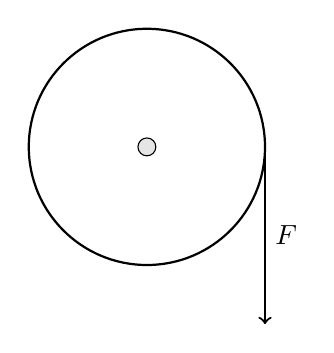
\begin{tikzpicture}[scale=0.75]
        \draw[fill=white!90!black] (0,0) circle (1ex);
        \draw[thick] (0,0) circle (2cm);
        \draw[thick,->] (2,0) -- ++(270:3) node[pos=0.5,anchor=west] {$F$};
    \end{tikzpicture}
    \end{center}
    The string is pulled with a force $F$ equal to the cylinders weight.
    What is the acceleration of the string?
    \begin{multicols}{3}
    \begin{choices}
      \correctchoice{$2g$}
        \wrongchoice{$g$}
        \wrongchoice{$\dfrac{g}{2}$}
        \wrongchoice{$\dfrac{g}{4}$}
        \wrongchoice{$\dfrac{F}{g}$}
    \end{choices}
    \end{multicols}
\end{question}
}


\endinput


